\NeedsTeXFormat{LaTeX2e}
\documentclass{jfp}
\usepackage{amssymb}
\usepackage{xcolor}
\usepackage{semantic}

\title{Composable data visualizations}
\author[Tomas Petricek]{TOMAS PETRICEK\\
       University of Kent, UK\\
       \email{t.petricek@kent.ac.uk}}

\definecolor{kvdclr}{rgb}{0.5,0.0,0.5}
\definecolor{fkvdclr}{rgb}{0.0,0.0,0.6}
\definecolor{urlclr}{rgb}{0.0,0.0,0.8}
\definecolor{idclr}{rgb}{0.0,0.0,0.0}
\definecolor{numclr}{rgb}{0.0,0.4,0.0}
\definecolor{strclr}{rgb}{0.6,0.2,0.0}

\newcommand{\lsep}{\;\;|\;\;}
\newcommand{\num}[1]{\textcolor{numclr}{#1}}
\newcommand{\str}[1]{\textnormal{\textcolor{strclr}{\sffamily "#1"}}}
\newcommand{\strf}[1]{\textnormal{\textcolor{strclr}{\sffamily #1}}}
\newcommand{\ident}[1]{\textnormal{\textcolor{idclr}{\sffamily #1}}}
\newcommand{\kvd}[1]{\textnormal{\textcolor{kvdclr}{\sffamily #1}}}
\newcommand{\fkvd}[1]{\textnormal{\textcolor{fkvdclr}{\sffamily #1}}}
\newcommand{\narrow}[1]{\hspace{-0.6em}#1\hspace{-0.6em}}
\newcommand{\urrl}[1]{\textnormal{\textcolor{urlclr}{\url{#1}}}}

\newcommand{\langl}{\begin{picture}(4.5,7)
\put(1.1,2.5){\rotatebox{60}{\line(1,0){5.5}}}
\put(1.1,2.5){\rotatebox{300}{\line(1,0){5.5}}}
\end{picture}}
\newcommand{\rangl}{\begin{picture}(4.5,7)
\put(.9,2.5){\rotatebox{120}{\line(1,0){5.5}}}
\put(.9,2.5){\rotatebox{240}{\line(1,0){5.5}}}
\end{picture}}

\begin{document}
\maketitle[f]

% \begin{abstract}
% This guide is for authors who are preparing papers for the \emph{Journal of
% Functional Programming} using the \LaTeXe\ document-preparation system
% and the Functional Programming class file (\texttt{jfp1.cls}).
% \end{abstract}


\section{Introduction}
Let's say we want to create the two charts in Figure~\ref{fig:charts}. The chart on the left is
a bar chart that shows two different values for each bar. The chart on the right consists of two
line charts that share the X axis with parts of the timeline highlighted using two different colors.

There is a plenty of libraries that can draw bar charts and line charts, but adding those extra
features will only be possible if the author already thought about your exact scenario.
Google Charts \cite{gcharts} supports the left chart (it is called Dual-X Bar Chart) but there is no
way for adding a background, or sharing an axis between charts. The alternative is to use a more
low-level library. In D3 \cite{d3} you construct the chart piece by piece, but you have to
tediously transform your values to coordinates in pixels yourself. For scientific plots,
you could use ggplot2 \cite{ggplot2}, based on the Grammar of Graphics \cite{grammar}.
A chart is a mapping from data to geometric objects (points, bars, lines) and their visual
properties (X and Y coordinate, shape, color). However, the range of charts that can be
created using this systematic approach is still somewhat limited.

What would an elegant functional approach to data visualization look like? A functional programmer
would want a domain-specific language that has a small number of primitives; allow us to define
high level abstractions such as a bar chart and its basic building blocks are expressed in terms
of domain values such as the exchange rate, rather than pixels.

\begin{figure}[h]
  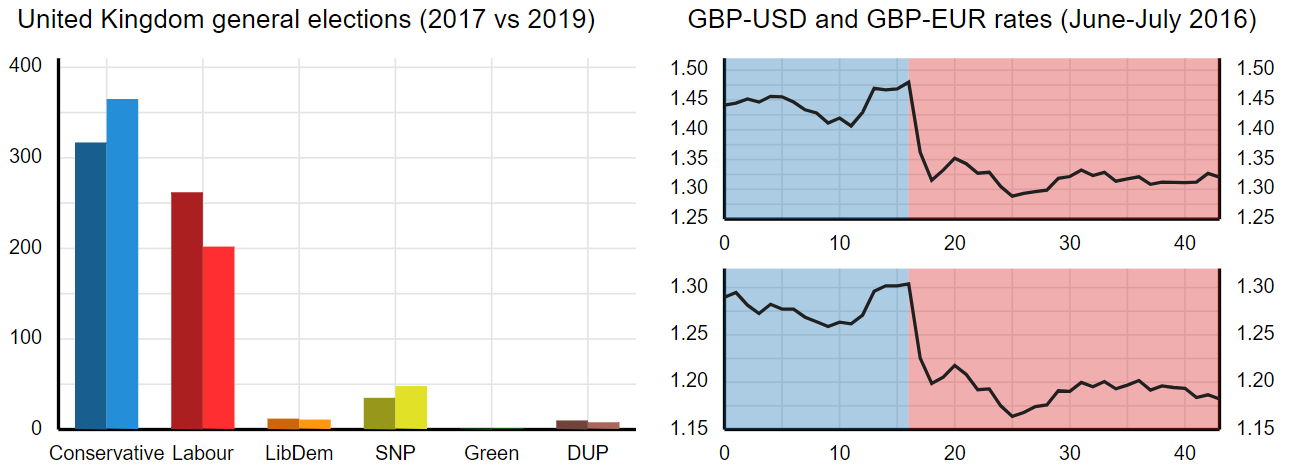
\includegraphics[scale=0.57]{figures/charts}
  \vspace{0.25em}
  \caption{Two charts about the UK politics: Comparison of election results from 2017 and 2019 (left)
    and GBP/USD exchange rate with highlighted areas before and after the 23 June 2016 Brexit vote.}
  \label{fig:charts}
\end{figure}

As is often the case with domain-specific languages, finding the right primitives is more of an art
than science. For this reason, we present an answer, a library named Compost, as a functional pearl.
We hope to convince the reader that Compost is elegant and we illustrate this with a wide range
of examples. Compost has a number of specific desirable properties:

\begin{itemize}
\item Charts are composed from a small number of primitive building blocks using a small number of
  combinators. In particular, concepts such as bar charts, line charts or charts with aligned
  axes are all expressed in terms of more basic concepts.
\item The primitives are specified in domain terms. When drawing a line, the value of an Y coordinate
  is an exchange rate of 1.36 USD/GBP, not 67 pixels from the bottom.
\item Most common chart types can be easily captured as high level abstractions, but there is an
  elengant way of creating a majority of more interesting custom charts.
\item The approach can easily be integrated with the Elm architecture \cite{elm}
	to creating web-based charts that involve animations or interaction with the user.
\end{itemize}
%
The presentation in this paper focuses on explaining the primitives and combinators of the
domain-specific language. We outline the structure of an implementation, but omit the details. Filling
those in requires careful thinking about geometry and projections, but there are no unexpected
surprises. A complete F\# implementation, including the examples used in this paper, is available
at: \urrl{http://github.com/compostjs}.

\section{Basic charts: Overlaying chart primitives}
We introduce individual features of the Compost library gradually. The first important aspect of
Compost is that properties of shapes are defined in terms of domain-specific values. In this
section, we explain what this means and then use domain-specific values to specify the core part of the
UK election results bar chart.

\begin{figure}[t]
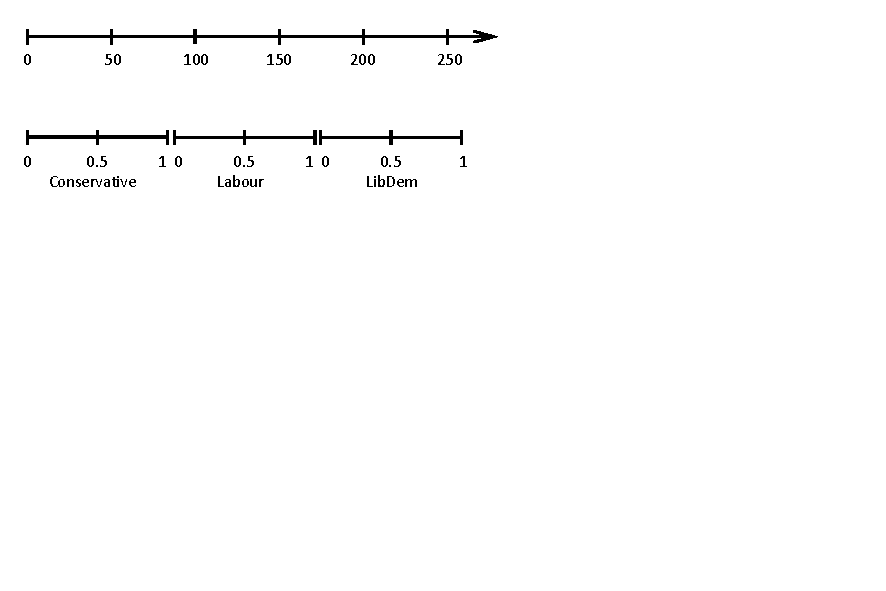
\includegraphics[scale=1,trim={0cm 6.5cm 6cm 0cm},clip]{figures/values.pdf}
\caption{On a continuous scale (above), an exact position is determined by a number.
  On a categorical scale (below), an exact position is determined by the category and a
  numerical ratio from 0 to 1.}
\label{fig:scales}
\end{figure}

\subsection{Domain-specific values}

In the election results chart in Figure~\ref{fig:charts} (left), the X axis shows categorical
values representing the political parties such as \strf{Conservative} or \strf{Labour}. The
Y axis shows numerical values representing the number of seats won such as $\num{365}$ MPs.
When creating data visualizations, those are the values that the user needs to specify. This is
akin to most high-level charting libraries such as Google Charts, but in contrast with more
flexible libraries like D3.

Our design focuses on two-dimensional charts with X and Y axes. Values mapped to those axes
can be either categorical (e.g.~political parties, countries) or continuous
(e.g.~number of votes, exchange rates). The mapping from categorical and continuous values
to positions on the chart is done automatically. For continuous values, this involves
applying a linear transformation. For categorical values, the mapping is more difficult.

For example, in the UK election results chart, the X axis is categorical. The library automatically
divides the available space between the six categorical values (political parties). The value
\strf{Green} does not determine an exact position on the axis, but rather a range. To determine
an exact position, we also need to attach a value between $\num{0}$ and $\num{1}$ to the
categorical value. This identifies a relative position in the available range.

Figure~\ref{fig:scales} illustrates the two kinds of values using the axes from the UK
election results chart. In Figure~\ref{fig:shape}, we define a value $v$ as either a continuous value
$\kvd{cont}~n$ containing any number $n$ or a categorical value $\kvd{cat}~c, r$, consisting
of a categorical value $c$ (implemented as a string) and a ratio $r$ between $0$ and $1$.
%
\begin{figure}
\begin{equation*}
\begin{array}{rcl}
v & = & \kvd{cat}~c, r \\
  & | & \kvd{cont}~n\\
  ~
\end{array}
\qquad
\begin{array}{rclcl}
s & = &\kvd{line}~\gamma, [\,v_{x1}, v_{y1}, \ldots, v_{xn}, v_{yn}\,] & | & \kvd{overlay}~[\,s_1, \ldots, s_n\,]\\
 & | & \kvd{fill}~\gamma, [\,v_{x1}, v_{y1}, \ldots, v_{xn}, v_{yn}\,] & | &\kvd{axis}_{l/r/t/b}~s\\
 & | & \kvd{text}~\gamma, v_x, v_y, t & | &\kvd{padding}~n_t,n_r,n_b,n_l,s\\
 & | & \kvd{bubble}~\gamma, v_x, v_y, w, h
\end{array}
\end{equation*}
\caption{Core primitives of the Compost domain-specific language. Values $v$ are either categorical
  or continuous; a shape $s$ is then defined as a simple recursive algebraic data type.}
\label{fig:shape}
\end{figure}

\subsection{Basic primitives and combinators}
\label{sec:basic-primitives}

Now that we know how Compost represents values, we can define the basic elements of its
domain-specific langauge. A chart is represeted by the shape $s$ defined in Figure~\ref{fig:shape}.
A primitive shape can be a text label, a line connecting a list of points, a filled polygon
defined by a list of points or a bubble at a given point with a given width and height.
The position of points is specified by X and Y coordinates, which can be either categorical or
continuous values. For text, line, polygon and bubble, we also include a parameter $\gamma$
that specifies the element color. The width and height of a bubble is given in pixels.

Figure~\ref{fig:shape} also defines three combinators. The most important is $\kvd{overlay}$,
which overlays all shapes from a given list. When doing this, Compost automatically infers the
scales of X and Y axes and calculates suitable projections using a method discussed in the next
section. Finally, $\kvd{padding}$ adds padding around a specified shape and $\kvd{axis}$ adds
an axis showing the inferred scale on the left, right, top or bottom of a given shape.
Using those primitives, we can construct the simple UK election results bar chart in Figure~\ref{fig:simple} (left).
We use the \fkvd{let} construct of the host functional language to structure the code:
%
\begin{equation*}
\begin{array}{l}
\fkvd{let}~\ident{conservative},~\ident{labour}~=\\
\quad \kvd{fill}~\strf{\#0000ff},
 ~[\;\,(\kvd{cat}~\strf{Conservative}, \num{0}), (\kvd{cont}~\num{0}), (\kvd{cat}~\strf{Conservative}, \num{0}), (\kvd{cont}~\num{365}),\\
\hspace{6.7em}\;(\kvd{cat}~\strf{Conservative}, \num{1}), (\kvd{cont}~\num{365}), (\kvd{cat}~\strf{Conservative}, \num{1}), (\kvd{cont}~\num{0})\;\,],\\
\quad \kvd{fill}~\strf{\#ff0000},
 ~[\;\,(\kvd{cat}~\strf{Labour}, \num{0}), (\kvd{cont}~\num{0}), (\kvd{cat}~\strf{Labour}, \num{0}), (\kvd{cont}~\num{202}),\\
\hspace{6.7em}\;(\kvd{cat}~\strf{Labour}, \num{1}), (\kvd{cont}~\num{202}), (\kvd{cat}~\strf{Labour}, \num{1}), (\kvd{cont}~\num{0})\,\;]\\[0.5em]
\kvd{axis}_l~(\kvd{axis}_b~(\kvd{overlay}~[~\ident{labour}, \ident{conservative}~]))\\
\end{array}
\end{equation*}

\noindent
The chart specification overlays two bars of different colors and then adds axes to the bottom and
left of the chart. The two bars are filled rectangles defined using four corner points. The Y
coordinates are specified as continuous values, while the X coordinates are categorical. For
the Conservative party, two of the points have the Y coordinate set to $\kvd{cont}~\num{0}$ (bottom of the bar)
and two have the Y coordinate set to $\kvd{cont}~\num{365}$ (top of the bar). The two X coordinates
are the start and the end of the range allocated for the \strf{Conservative} category,
i.e.~$\kvd{cat}~\strf{Conservative}, \num{0}$ on the left and $\kvd{cat}~\strf{Conservative}, \num{1}$
on the right.

\begin{figure}
  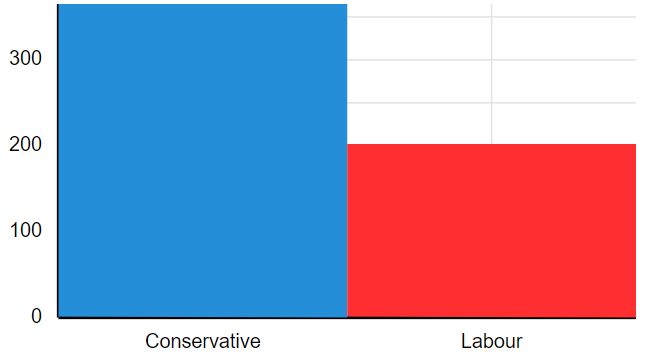
\includegraphics[scale=0.57]{figures/simple}
  \vspace{0.25em}
  \caption{Simple chart showing the UK election results; using automatically inferred scales (left)
    and using rounded Y scale and explicitly defined (reordered) X scale (right).}
  \label{fig:simple}
\end{figure}

Extending the snippet to generate a grouped bar chart that shows two results
for each party as in Figure~\ref{fig:charts} is easy. Given a party $p$, we need to
generate two rectangles, one with X coordinates $\kvd{cat}~p, 0$ and $\kvd{cat}~p, 0.5$
and the other with X coordinates $\kvd{cat}~p, 0.5$ and $\kvd{cat}~p, 1$.
In the following snippet, we use a \fkvd{for} comprehension to generate the list. All remaining
constructs are primitives of the Compost domain-specific language. Assuming \ident{elections} is a
list of election results containing a five-element tuple consisting of a party name, colors for
2017 and 2019 and results for 2017 and 2019 we create the chart using:
%
\begin{equation*}
\begin{array}{l}
  \kvd{axis}_l~(\kvd{axis}_b~(\kvd{overlay}~[\\
  \quad \fkvd{for}~\ident{party}, \ident{clr17}, \ident{clr19}, \ident{mp17}, \ident{mp19}~\fkvd{in}~\ident{elections}~\rightarrow\\
  \quad\quad \kvd{padding}~0,10,0,10,\,\kvd{overlay}~[\\
  \quad\quad\quad \kvd{fill}~\ident{clr17},~[\,(\kvd{cat}~\ident{party}, \num{0}), (\kvd{cont}~\num{0}), (\kvd{cat}~\ident{party}, \num{0}), (\kvd{cont}~\ident{mp17}),\\
  \quad\quad\quad \hspace{4.08em}           ~(\kvd{cat}~\ident{party}, \num{0.5}), (\kvd{cont}~\ident{mp17}), (\kvd{cat}~\ident{party}, \num{0.5}), (\kvd{cont}~\num{0}) \,], \\
  \quad\quad\quad \kvd{fill}~\ident{clr19},~[\,(\kvd{cat}~\ident{party}, \num{0.5}), (\kvd{cont}~\num{0}), (\kvd{cat}~\ident{party}, \num{0.5}), (\kvd{cont}~\ident{mp19}),\\
  \quad\quad\quad \hspace{4.08em}           ~(\kvd{cat}~\ident{party}, \num{1}), (\kvd{cont}~\ident{mp19}), (\kvd{cat}~\ident{party}, \num{1}), (\kvd{cont}~\num{0})\,]~~]~~]\,)\,)\\
\end{array}
\end{equation*}

\noindent
Aside from iterating over all available parties and splitting the bar, the example also adds padding
around the bars. A padding is specified in pixels rather than in terms of domain values. This is
sometimes preferrable over, for example, drawing a bar using a range from $\num{0.05}$ to $\num{0.5}$.
The chart is still missing a title, which we add in Section~\ref{sec:abstractions}.

\subsection{Inferring scales and projections}
\label{sec:basic-scales}

When composing shapes using the \kvd{overlay} primitive, the user does not need to specify how
to position the child elements relatively to each other. The Compost library positions the elements
automatically. This is done in two steps. First, Compost infers the \emph{scales} for X and Y
axes. A scale represents the range of values that needs to fit in the space available for the chart.
Second, Compost calculates a \emph{projection}, a mapping from domain-specific values of the scale
to the available screen space. A scale $l$ is defined in Figure~\ref{fig:scale}.

\begin{figure}
\vspace{-0.5em}
\begin{equation*}
\begin{array}{rcl}
l & = & \kvd{continuous}~n_{min}, n_{max} \lsep \kvd{categorical}~[\,c_1, \ldots, c_k\,]
\end{array}
\end{equation*}
\vspace{-1em}
\caption{A scale $l$ can be continuous, defined by a range, or categorical, defined by a list of values.}
\label{fig:scale}
\vspace{-1em}
\end{figure}
\begin{figure}
\begin{equation*}
\begin{array}{rclcl}
s & = & \kvd{roundScale}_{x/y} s      &|& \kvd{nest}_{x/y}~v_{min}, v_{max}, s \\
  & | & \kvd{explicitScale}_{x/y}~l, s &|&  (\ldots)
\end{array}
\end{equation*}
\caption{Additional combinators for controlling and nesting scales, extending earlier definition of $s$.}
\label{fig:control}
\end{figure}

A continuous scale is defined by a minimal and maximal value that need to be mapped to the
available chart space. A categorical scale is defined by a list of individual categorical values.
Note that we do not need a minimal and maximal ratios of the used categorical values as Compost
will use an equal space for each category, regardless of where in this space a shape needs to
appear.

Inferring scales is done by a simple recursive function that walks over the given shape and
constructs two scales for the X and Y axis, using the X and Y coordinates that appear in the shape.
Most of the work is done by a simple helper function that takes two scales, $l_1$ and $l_2$,
and produces a new scale that represents the union of the two:
%
\begin{equation*}
\begin{array}{l}
\ident{union}~(\kvd{continuous}~n_l, n_h)~(\kvd{continuous}~n'_l, n'_h) =\\
\qquad\kvd{continuous}~\min(n_l, n'_l), \max(n_h, n'_h)\\[0.5em]
\ident{union}~(\kvd{categorical}~[\,c_1, \ldots, c_p\,])~(\kvd{categorical}~[\,c'_1, \ldots, c'_q\,]) =\\
\qquad \kvd{categorical}~[\,c_1, \ldots, c_p\,] \;@\; [\,c'_i~|~ \forall i\in 1\ldots q, \nexists j. c_j = c'_i \;]
\end{array}
\end{equation*}

\vspace{-0.5em}
\noindent
When unioning two continuous scales, the minimum and maximum of the resulting scale is the smallest
and largest of the two minimums and maximums, respectively. When unioning two categorical scales,
we take all values of the first scale and append all values of the second scale that do not appear
in the first one. Note that this means that the order of categorical values in a scale depends on
the order in which they appear in the shape. (A possible improvement to Compost would be to support
ordinal values, which are categorical values with a well-defined ordering.) It is also worth noting
that a categorical scale cannot be combined with a continuous scale. In other words, mixing
categorical and continuous values in a single scale results in an error.

Once Compost computes scales for a given shape and its sub-shapes, it constructs a projection
that maps domain-specific values to the available chart space. We discuss this in
Section~\ref{sec:impl}. For a continuous scale, the projection is a linear transformation. For
categorical scale with $k$ values, we split the available chart space into $k$ equally sized
regions and then map a categorical value $\kvd{cat}~c, r$ to the region corresponding to $c$
according to the ratio $r$.

\subsection{Types and units of measure}
We introduce the Compost domain-specific language as untyped, but there are some obvious ways in
which types could make composing charts in Compost safer. First, a type representing a shape could
specify whether the X and Y axes represent categorical or continous values. This would rule out
mixing of different values on a single scale and guarantee that the \ident{union} operation,
sketched in the previous section, is never called in a way leading to an undefined result.
Second, the type of values mapped to an axis could be further annotated with units of measure
\cite{units}. Using the F\# notation where $n\langl u\rangl$ is a number $n$ with unit $u$,
an axis containing a value $\kvd{cont}~\num{317}\langl \ident{mp}\rangl$ would then be incompatible
with an axis containing a value $\kvd{cont}~\num{1.32}\langl \ident{gbp}/\ident{usd}\rangl$.

The design of the type system for Compost is straightforward, so we only present a brief sketch.
There are two kinds of types; $\sigma$ is a type of values and $\tau$ is a type of shapes.
Assuming $u$ denotes a unit of measure, the types are defined as:
%
\begin{equation*}
\begin{array}{rcl}
\sigma & = & \kvd{Cat}~u \lsep \kvd{Cont}~u
\end{array}
\qquad\qquad
\begin{array}{rcl}
\tau & = & \kvd{Shape}~\sigma_x, \sigma_y \\
\end{array}
\end{equation*}

\vspace{-1em}
\noindent
Correspondingly, there are two kinds of judgements; $v\vdash \sigma$ indicates the type of a
value, while $s\vdash \tau$ indicates the type of a shape. The typing rules for two of the
basic chart primitives, \kvd{line} and \kvd{overlay} look as follows:
%
\begin{equation*}
\inference
  {v_{xi} \vdash \sigma_x & v_{yi} \vdash \sigma_y}
  {\kvd{line}~\gamma, [\,v_{x1}, v_{y1}, \ldots, v_{xn}, v_{yn}\,] \vdash \kvd{Shape}~\sigma_x, \sigma_y}
\qquad
\inference
  {s_i \vdash \kvd{Shape}~\sigma_x, \sigma_y}
  {\kvd{overlay}~[\,s_1, \ldots, s_n\,] \vdash \kvd{Shape}~\sigma_x, \sigma_y}
\end{equation*}

\vspace{-0.5em}
\noindent
The rule for \kvd{line} ensures that all X and Y values have the same types, $\sigma_x$ and $\sigma_y$,
respectively and infers $\kvd{Shape}~\sigma_x, \sigma_y$ as the type of the shape. The rule for
\kvd{overlay} ensures that all composed shapes have the same type, including the type of X and Y scales.



\section{Advanced charts: Controlling scale composition}
\label{sec:fancy}

Most charts have one X and one Y axis that are determined by the values the chart shows,
but there are interesting exceptions. The chart in Figure~\ref{fig:charts} (right)
has two different Y axes, one for GBP/USD and one for GBP/EUR. In the next two sections, we look at
three combinators that control the scale inferrence process and what flexibility this enables.

\subsection{Defining nice scale ranges}

The automatic scale inference often results in scales where the maximum is a non-round number.
This leads to charts that fully utilize the available space, but may not be easy to read.
The first two primitives, shown in Figure~\ref{fig:control} (left) allow the chart designer
to adjust the automatically inferred range of scales.

The two combinators for controlling the range of scales are \kvd{roundScale} and \kvd{explicitScale}.
The oprations can be applied to either the X scale or the Y scale, which is indicated by the
$x/y$ sub-script. The \kvd{roundScale} primitve takes the inferred X or Y scale of the shape $s$
and, if it is a continuous scale, rounds its minimal and maximal values to a ``nice'' number.
For example, if a continuous scale has minimum $\num{0}$ and maximum $\num{365}$, the resulting
scale would have a maximum $\num{400}$. For categorical scale, the operation does not have any effect.
The \kvd{explicitScale} operation is similar, but it replaces the inferred scale with an explicitly
provided scale (the type of the inferred scale has to match with the type of the explicitly given
scale). For example, the chart in Figure~\ref{fig:simple} (right) is constructed using the
following code (reusing the \ident{labour} and \ident{conservative} variables defined earlier):
%
\begin{equation*}
\begin{array}{l}
\kvd{axis}_l~(\kvd{axis}_b~(\kvd{roundScale}_y~(\kvd{explicitScale}_x~(\kvd{categorical}~[\,\strf{Labour},\strf{Conservative}\,]),\\
\qquad \kvd{overlay}~[~\ident{labour}, \ident{conservative}~]~)))\\
\end{array}
\end{equation*}
\vspace{-0.5em}

\noindent
Reading the code from the inside out, the snippet first overlays the two coloured bars defined
earlier; it then replaces the X axis with an explicitly given one that changes the order of the
values. As a result, the bar for \strf{Labour} will appear on the left, even though the value
comes later in the list of overlaid chart elements.

The code next uses \kvd{roundScale} to automatically round the minimum and maximum of the
continuous Y scale (showing the total number of seats). Finally, we add axes around the shape,
producing a usual labelled chart.  It is worth noting that \kvd{axis} and \kvd{roundScale}
could be implemented as derived operations; \kvd{roundScale} would need to infer the scale of
the nested shape and then insert \kvd{explicitScale} with a rounded number; \kvd{axis}
would also need to infer the scales and then generates labels and lines in suitable locations.

\begin{figure}
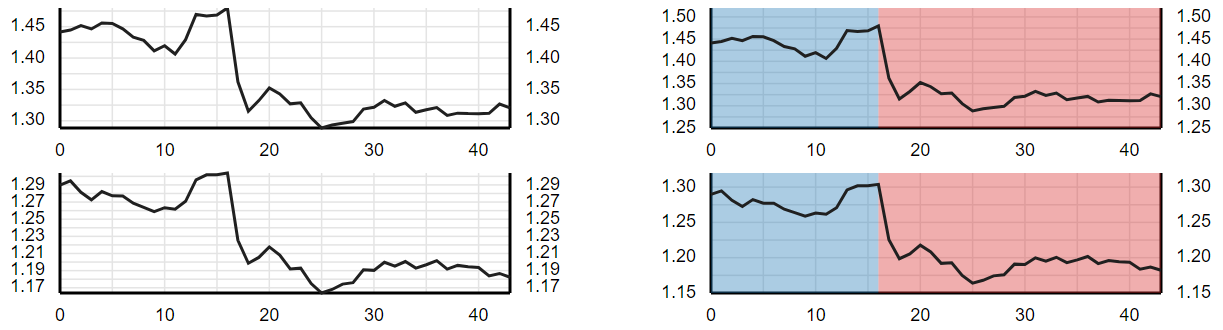
\includegraphics[scale=0.57]{figures/lines}
\vspace{0.25em}
\caption{Two charts showing currency exchange rates with a shared X scale and separate Y scales.}
\label{fig:lines}
\end{figure}

\subsection{Nested scales}

The most interesting primitive for controlling scale composition defined in Figure~\ref{fig:control}
is $\kvd{nest}_{x/y}$. The combinator takes two values, $v_{min}, v_{max}$ and a shape $s$ as arguments
and it nests the scale of the shape $s$ inside the region defined by $v_{min}, v_{max}$. When inferring
scales of shapes, the scale of $\kvd{nest}_{x/y}~l, s$ will be a categorical or continuous scale
inferred using the values $v_{min}$ and $v_{max}$, regardless of the values that are used inside
the shape $s$. The chart space between $v_{max}$ and $v_{min}$ will then be used to render the
nested shape $s$ using its inferred scale. An example of nesting is shown in Figure~\ref{fig:nesting}.
Here, a chart with a continous scale from $\num{1.1}$ to $\num{1.4}$ (e.g.~GBP/EUR exchange rates)
is nested in the left half of another chart, which has a continuous scale from $\num{0}$ to $\num{100}$.

\begin{figure}
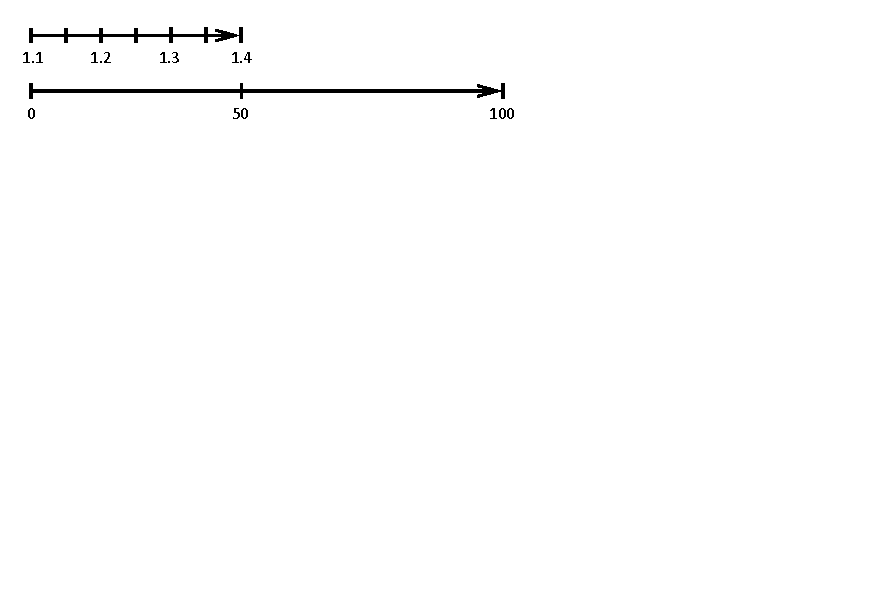
\includegraphics[scale=1,trim={0cm 7.5cm 6cm 0cm},clip]{figures/nest}
\caption{A continuous scale with values from $0$ to $6$, nested in another scale.}
\label{fig:nesting}
\end{figure}

The nesting of scales can be used in a variety of ways. We can, for example, nest a line chart
inside a bar of a bar chart. In that case, the values for $v_{min}$ and $v_{max}$ would be
$\kvd{cat}~\strf{ABC}, 0$ and $\kvd{cat}~\strf{ABC}, 1$, which define the start and the end of
the region allocated to the $\strf{ABC}$ category on a categorical scale. A simpler use case for
the combinator is showing multiple charts in a single view. For example, the motivating example
in Figure~\ref{fig:charts} (right) comapres aligned line charts of exchange rates for two
different currencies. Assuming \ident{gbpusd} and \ident{gbpeur} are lists containing days as X
values and exchange rates as Y values, we can construct a simple chart with two line charts,
shown in Figure~\ref{fig:lines} (left), using:
%
\begin{equation*}
\begin{array}{l}
\kvd{overlay}~[~
\kvd{nest}_y~(\kvd{cont}~\num{0}),(\kvd{cont}~\num{50}), (\kvd{axis}_l~(\kvd{axis}_r~(\kvd{axis}_b~(\kvd{line}~\strf{\#202020}~\ident{gbpusd}))))\\
\hspace{3.68em} \kvd{nest}_y~(\kvd{cont}~\num{50}),(\kvd{cont}~\num{100}), (\kvd{axis}_l~(\kvd{axis}_r~(\kvd{axis}_b~(\kvd{line}~\strf{\#202020}~\ident{gbpeur}))))~]\\
\end{array}
\end{equation*}

\vspace{-0.5em}
\noindent
In this example, the X scale shows the days of the year. This scale is shared by both of the charts.
Indeed, if data was only available for the second half of the month for one of the charts,
we would want the line to start in the middle of the chart. However, the Y scale needs to be
separate for each of the charts. To achieve this, we use $\kvd{nest}_y$. The scale of the inner
shapes is continuous, from the minimal to the maximal exchange rate for a given period. The
outer scale is determined by the explicitly defined points. For the upper chart, these are
$\kvd{cont}~\num{0}$ and $\kvd{cont}~\num{50}$; for the lower chart, these are
$\kvd{cont}~\num{50}$ and $\kvd{cont}~\num{100}$. The continuous values define a scale that only
contain two shapes -- one in the upper half, one in the lower half -- and so the three numbers could
have equally been, for example, $\num{0},\num{1}, \num{2}$. The outer scale used here is
synthetic and it is not aligned with other chart elements. An example of a more complex chart
that follows a similar style, but does not have synthetic outer scale would be pairplot from
the seaborn Python library \cite{seaborn}.

For completeness, the following code snippet shows how to construct the full currency exchange
rate chart shown in Figure~\ref{fig:lines} (right), including the blue and red background:
%
\begin{equation*}
\begin{array}{l}
\fkvd{let}~\ident{xrate}~(\ident{lo}, \ident{hi})~\ident{rates}~=\kvd{overlay}~[\\
\quad \kvd{fill}~\strf{\#1F77B460}, [\;\,\kvd{cont}~\num{0}, \kvd{cont}~\ident{lo}, \kvd{cont}~\num{16}, \kvd{cont}~\ident{lo}, \kvd{cont}~\num{16}, \kvd{cont}~\ident{hi}, \kvd{cont}~\num{0}, \kvd{cont}~\ident{hi}\;],\\
\quad \kvd{fill}~\strf{\#D6272860}, [\;\,\kvd{cont}~\num{16}, \kvd{cont}~\ident{lo}, \kvd{cont}~\num{44}, \kvd{cont}~\ident{lo}, \kvd{cont}~\num{44}, \kvd{cont}~\ident{hi}, \kvd{cont}~\num{16}, \kvd{cont}~\ident{hi}\;],\\
\quad \kvd{line}~\strf{\#202020}~\ident{rates}~]\\[0.5em]
\kvd{overlay}~[~
\kvd{nest}_y~(\kvd{cont}~\num{0}),(\kvd{cont}~\num{50}), (\kvd{axis}_l~(\kvd{axis}_r~(\kvd{axis}_b~(\ident{xrate}~(\num{1.25}, \num{1.50})~\ident{gbpusd}))))\\
\hspace{3.68em} \kvd{nest}_y~(\kvd{cont}~\num{50}),(\kvd{cont}~\num{100}), (\kvd{axis}_l~(\kvd{axis}_r~(\kvd{axis}_b~(\ident{xrate}~(\num{1.15}, \num{1.30})~\ident{gbpeur}))))~]\\
\end{array}
\end{equation*}

\noindent
Here, we use the \fkvd{let} binding of the host language to define a function that takes
a the data \ident{rates} together with the minimum and maximum. This is used for drawing
two filled rectangles, covering the first 16 days of the view in blue and the rest in red.
The shapes combined using \kvd{overlay} are rendered in the order in which they appear and so
the line shape is last, so that it appears above the background.

\begin{figure}
  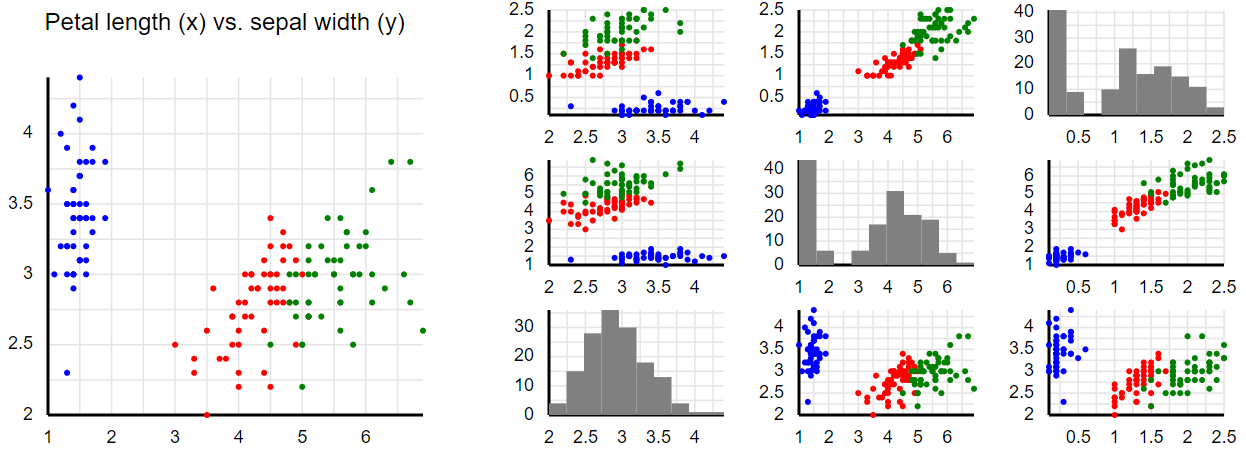
\includegraphics[scale=0.57]{figures/standard}
  \vspace{0.25em}
  \caption{Sample charts built using derived abstractions; a scatter plot visualizing the Iris\\
    dataset with a title (left) and a pairplot comparing two Iris features (right).}
  \label{fig:standard}
\end{figure}

\section{Standard charts: Definining new abstractions}
\label{sec:abstractions}

The Compost library does not introduce a rich collection of standard charts and chart features
as most charting libraries. However, the functional domain-specific language design makes
it easy to define high-level chart features based on the low-level primitives of the core language.
To illustrate this, we give two examples.

First, one last remaining feature of the two charts in Figure~\ref{fig:charts} is a chart title.
This can be added to any chart using the following derived combinator:
%
\begin{equation*}
\begin{array}{l}
\fkvd{let}~\ident{title}~t~s~=\kvd{overlay}~[\\
\quad \kvd{nest}_x~(\kvd{cont}~\num{0}), (\kvd{cont}~\num{100}),
  (\kvd{nest}_y~(\kvd{cont}~\num{0}), (\kvd{cont}~\num{15}), \\
\quad\quad \kvd{explicitScale}_x~(\kvd{continuous}~\num{0},\num{100}),~(\kvd{explicitScale}_y~(\kvd{continuous}~\num{0},\num{100}),\\
\quad\qquad \kvd{text}~\strf{\#000000}, (\kvd{cont}~\num{50}), (\kvd{cont}~\num{50}),~t)~)\\
\quad \kvd{nest}_x~(\kvd{cont}~\num{0}), (\kvd{cont}~\num{100}),
  (\kvd{nest}_y~(\kvd{cont}~\num{15}), (\kvd{cont}~\num{100}),~s)~]
\end{array}
\end{equation*}

\vspace{-0.5em}
\noindent
The \ident{title} combinator is a function defined using \fkvd{let} in the host language. It takes
a title $t$ and a shape $s$. It overlays two shapes. To position the title above the chart, the first
shape has an outer Y scale $\kvd{continuous}~\num{0},\num{15}$ while the second has an outer Y scale
$\kvd{continuous}~\num{15},\num{100}$. These are defined using the $\kvd{nest}_y$ primitive. Similarly,
the outer X scale of both is $\kvd{continuous}~\num{0},\num{100}$, defined using $\kvd{nest}_x$.

The second shape simply wraps the specified chart $s$ to which we are attaching the title. The first
positions the text title in the middle of the available space. To do so, we explicitly set the X and
Y scales inside the upper shape to continuous scales from $\num{0}$ to $\num{100}$ and then position
the text label in the middle, at a point $(\kvd{cont}~\num{50}), (\kvd{cont}~\num{50})$.
Figure~\ref{fig:standard} (left) shows a sample scatter plot chart with a title created using the
\ident{title} combinator.

A more complex type of chart that can be easily composed using the Compost primitives is the
pairplot chart from the seaborn library \cite{seaborn}.
Pairplot visualizes pairwise relationships between features of a dataset.
An example using three features (sepal width, petal width, petal length) from the Iris dataset is shown
in Figure~\ref{fig:standard} (right).
A pairplot draws a grid of charts, each visualizing the relationship between two numerical features. For distinct
features, pairplot shows a scatter plot using one fature for X values and the other for Y values.
At the diagonal (when the fatures are the same), it draws a histogram of the values of the feature.
Additionally, a categorical feature can be used to determine the color of dots in the scatter plots.

To generate a pairplot, we use \kvd{nest} to overlay and align a grid of plots. Each of those
overlays a number of bubbles or filled shapes and adds left and bottom axis. As before, we use
\fkvd{let} to define a function and list comprehensions to generate individual chart elements.
We assume that \ident{data} is a list of rows, \ident{attrs} is a list of available attributes and
$\ident{get}~a~r$ obtains the attribute $a$ of a row $r$. We also assume the dataset contains the \str{color} attribute.
%
\begin{equation*}
\begin{array}{l}
\fkvd{let}~\ident{pairplot}~\ident{attrs}~\ident{data}~=~\kvd{overlay}~[\\
\quad \fkvd{for}~x~\fkvd{in}~\ident{attrs}~\rightarrow~\fkvd{for}~y~\fkvd{in}~\ident{attrs}~\rightarrow\\
\qquad \kvd{nest}_x~(\kvd{cat}~x, 0), (\kvd{cat}~x, 1), (\kvd{nest}_y~(\kvd{cat}~y, 0), (\kvd{cat}~y, 1), \kvd{axis}_l~(\kvd{axis}_b\\
\quad\qquad (~\fkvd{if}~x \neq y~\fkvd{then}~\kvd{overlay}~[\;\fkvd{for}~r~\fkvd{in}~\ident{data}~\rightarrow~\\
\qquad\qquad \hspace{0.7em} \kvd{bubble}~(\ident{get}~\str{color}~r),~(\ident{get}~x~r), (\ident{get}~y~r), \num{1}, \num{1}~]\\
 \quad\qquad \hspace{0.7em} \fkvd{else}~\kvd{overlay}~[\;\fkvd{for}~x_1, x_2, y~\fkvd{in}~\ident{bins}~x~\ident{data}~\rightarrow~\\
\qquad\qquad \hspace{0.7em}  \kvd{fill}~\strf{\#808080}~[\; x_1, y, x_2, y, x_2, \num{0}, x_1, \num {0}\;]\;])))] \\
\end{array}
\end{equation*}

\vspace{-0.5em}
\noindent
As before, \kvd{nest} is essential for composing individual charts. Here, the points that determine
the locations of individual charts are categorical values defined by the attributes of the dataset.
The choice between two possible nested charts is made using the host language \fkvd{if} construct.
Scatter plots are generated by overlaying bubbles with X and Y coordinates obtained using $\ident{get}~x~r$
and $\ident{get}~y~r$. Histograms are composed from filled shapes. To obtain their locations, we use
a helper function $\ident{bins}~x~\ident{data}$, which returns a list of bins specified by a tripple
consisting of a lower and an upper range $x_1, x_2$ and the count $y$.

The example shows that the Compost is simple yet expressive. With just
a few lines of code, we are able to construct charts that, in other systems, require dedicated
libraries. The essential aspect of the language making this possible is the automatic inference
of scales and their mapping to the available space as well as the \kvd{nest} operation.


\section{Interactive charts: Domain-specific event handling}
Data visualizations published on the web often also feature interactivity. Standard forms of
interactivity include animations, hover labels or zooming. More interesting custom forms
include the ``You draw It'' visualization introduced by the New York Times \cite{youdraw}.
The chart shows only the first half of the data, such as a timeline, and the reader has to
guess the second half before clicking a button and seeing the actual data. Standard forms of
interactivity are supported by high-level libraries. For example, Google Charts supports panning
using drag \& drop, zooming to a selected chart range and animations. Custom interactivity can be
implemented using low-level libraries such as D3, but doing so requires directly handling
JavaScript events and modifying the browser DOM.

\subsection{Domain-specific events}
Compost can be used in conjunction with a virtual-dom library to create interactive data
visualizations based on the Elm architecture \cite{mvu}. An interactive visualization is described using
a pair of functions -- the \emph{view} function creates a chart based on the current state and
the \emph{update} function specifies how the state changes when an event occurs.

To support handling of mouse-based events, Compost adds three additional primitives to the definition
of shape, shown in Figure~\ref{fig:mouse}. The three new primitives make it possible to handle
three common mouse events using custom functions $\lambda \;x~y\rightarrow e$, specified in the
host language. The most interesting aspect is that the functions are given X and Y coordinates
of the event specified in the domain of the chart. This means that if the user clicks on the
bar representing the Conservative party in a bar chart, the values might be, for example,
$\kvd{cat}~\strf{Conservative},\num{0.75}$ for X and $\kvd{cont}~\num{120.5}$ for Y.

\end{figure}
\begin{figure}
\begin{equation*}
\begin{array}{rclcl}
s & = & \kvd{mouseUp}~(\lambda \,x~y \rightarrow e), s  &|& \kvd{mouseDown}~(\lambda \,x~y\rightarrow e), s  \\
    &|& \kvd{mouseMove}~(\lambda \,x~y \rightarrow e), s &|& (\ldots)
\end{array}
\end{equation*}
\caption{Additional combinators for mouse-based interaction, extending earlier definition of $s$.}
\vspace{0.5em}
\label{fig:mouse}
\end{figure}

\subsection{You draw it data visualizations}
To illustrate building of interactive data visualizations using Compost, we look at one aspect of
the ``You draw It'' visualizations. We want to create a bar chart where the user can use drag \& drop
to move individual bars. The resulting chart can be seen in Figure~\ref{fig:youdraw}.
The first step is to define types representing the state and events that can occur:
%
\begin{equation*}
\begin{array}{lll}
\fkvd{type}~\ident{State} &\narrow{=}& \ident{bool}~*~(\ident{string}~*~\ident{int})~\ident{list}\\[0.5em]
\fkvd{type}~\ident{Event} &\narrow{=}& \ident{Update}~\fkvd{of}~(\ident{string}~*~\ident{int})\\
                          &\;\narrow{|}& \ident{Moving}~\fkvd{of}~\ident{bool}
\end{array}
\end{equation*}

\vspace{-0.5em}
\noindent
The state is a pair of boolean, indicating whether the user is currently dragging, together with
a list of key value pairs, storing the number of seats for each political party. Two types of events
can occur in the visualization. First, the user may start or stop dragging, which is indicated using
$\ident{Moving}(\fkvd{true})$ and $\ident{Moving}(\fkvd{false})$, respectively. Second, the user
may change a value for a party, which is captured by the $\ident{Update}$ event.

The next part of the visualization is the \ident{update} function which takes an old state together
with an event and produces a new state:
%
\begin{equation*}
\begin{array}{l}
\fkvd{let}~\ident{update}~(\_,s)~(\ident{Moving}(m)) = m,s\\
\hspace{1.05em}~\ident{update}~(\fkvd{true},s)~(\ident{Update}(p, v)) =\\
\hspace{1.05em}\qquad  \fkvd{true}, \ident{map}~(\lambda(k, o) \rightarrow k, \fkvd{if}~k = p~\fkvd{then}~v~\fkvd{else}~o)~s\\
\hspace{1.05em}~\ident{update}~(m,s)~(\ident{Update}(\_, \_)) = m,s\\
\end{array}
\end{equation*}

\vspace{-0.5em}
\noindent
The first two cases handle the \ident{Update} event. The event carries two values, $p, v$, which
represent the party (which bar the user is dragging) and the new value (new number of seats).
If the user is currently dragging, we replace the value associated with the party $p$ in \newpage \noindent the
list $s$ using the \ident{map} function. If the user is not currently dragging, the event is ingored.
The last case handles the \ident{Moving} event, which simply replaces the first component of the
state tuple, i.e.~a flag indicating whether a mouse button is down.


\begin{figure}[t]
  \vspace{0.5em}
  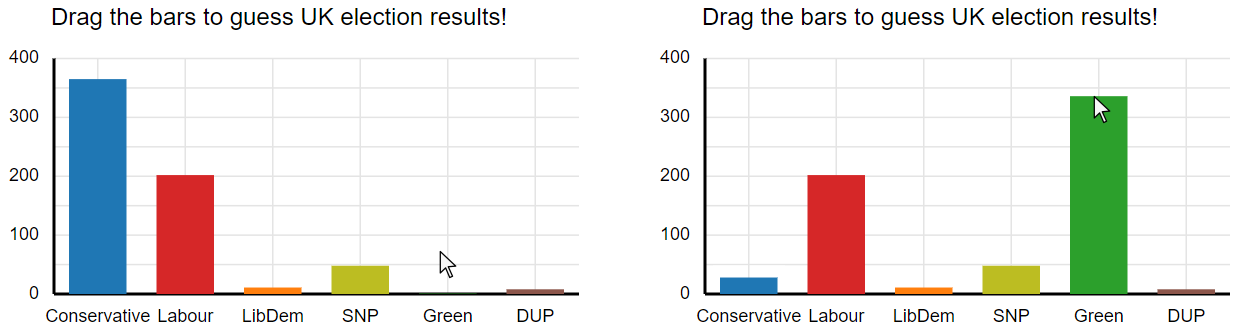
\includegraphics[scale=0.57]{figures/youdraw}
  \vspace{1em}
  \caption{Interactive ``You draw it'' data visualization. The user moves cursor to a bar (left),
    pushes a mouse button and drags the bar to the position that they think is the correct one (right).}
  \label{fig:youdraw}
\end{figure}

Finally, the \ident{render} function takes the current state and builds the data visualization
using the Compost domain-specific language. In addition, it also takes a parameter \ident{trigger},
which is a function of type $\ident{Event}\rightarrow\ident{unit}$ that can be used to trigger
events in handlers, registered using primitives such as \kvd{mouseMove}.
To build the bar chart in Figure~\ref{fig:youdraw}, we use the same approach as in
Section~\ref{sec:basic-primitives}. The only addition are the event handlers registered using
\kvd{mouseMove}, \kvd{mouseUp} and \kvd{mouseDown}:
%
\begin{equation*}
\begin{array}{l}
\fkvd{let}~\ident{render}~\ident{trigger}~(\_, \ident{state})~=\\
\quad \kvd{axis}_l~(\kvd{axis}_b~(\kvd{explicitScale}_y~(\kvd{continuous}~\num{0},\num{400}),\\
\qquad (~\kvd{mouseMove}~(\lambda \,(\kvd{cat}~p,\_)~(\kvd{cont}~v)\rightarrow \ident{trigger}(\ident{Update}(p, v))),\\
\qquad (~\kvd{mouseUp}~(\lambda \,\_~\_\rightarrow \ident{trigger}(\ident{Moving}(\fkvd{true}))),\\
\qquad (~\kvd{mouseDown}~(\lambda \,\_~\_\rightarrow \ident{trigger}(\ident{Moving}(\fkvd{false}))),~\kvd{overlay}~[\\
\qquad \qquad \fkvd{for}~\ident{party}, \ident{mps}~\fkvd{in}~\ident{state}~\rightarrow~\kvd{padding}~0,10,0,10,~(\kvd{fill}~(\ident{color}~\ident{party}),\\
\qquad \qquad\quad\quad [\,(\kvd{cat}~\ident{party}, \num{0}), (\kvd{cont}~\num{0}), (\kvd{cat}~\ident{party}, \num{0}), (\kvd{cont}~\ident{mp}),\\
\qquad \qquad\quad\quad \hspace{0.38em}(\kvd{cat}~\ident{party}, \num{0.5}), (\kvd{cont}~\ident{mps}), (\kvd{cat}~\ident{party}, \num{0.5}), (\kvd{cont}~\num{0}) \,])~~])))))\\
\end{array}
\end{equation*}

\vspace{-0.5em}
\noindent
When the user interacts with the visualization created using Compost, the library
translates the coordinates associated with events from pixels to domain-specific
values. In case of the above bar chart, when the user moves a mouse, the function registed
using \kvd{mouseMove} is given a categorical value $\kvd{cat}~p, r$ as the X coordinate and
a continuous value $\kvd{cont}~v$ as the Y coordinate. It then takes $p$, which is the name
of the party corresponding to the bar and the value $v$ corresponding to the number of seats
and triggers the $\ident{Update}(p, v)$ event to update the state. The handlers for
\kvd{mouseUp} and \kvd{mouseDown} do not use the coordinates. They simply switch the flag
indicating whether the user is currently dragging or not.

The pair of functions, \ident{update} and \ident{render}, together with an initial state is
all that is needed to create an interactive data visualization. Compost calls
\ident{render} each time the state changes and uses virtual-dom to update the chart
displayed in the browser. Although creating an interactive visualization is more work than
creating a static one, the domain-specific nature of Compost is invaluable. We can
simply take the values $p$ and $v$ produced by a mouse event, use those to update the state
and then, again, render an updated chart.


\section{Implementation structure: Scale inference and projection}
\label{sec:impl}

Compost is an open-source library, implmented in the functional language F\#. The full source
code can be found at \urrl{http://github.com/compostjs}.
As is often the case with functional domain-specific languages, the implementation is easy once
we find the right collection of basic primitives and the right structure for the implementation.
This largely applies to the Compost library and so we will not go into the implementation details.
It is, however, worth giving an outline of the implmentation structure.

As mentioned in Section~\ref{sec:basic-scales}, the rendering of shapes proceeds in two stages.
First, the library infers the scales of a shape. When doing so, it also annotates some shapes
with additional information that are needed later for rendering. Second, the library projects
the shape onto an available space and produces the chart, represented as an SVG object.

\subsection{Inferring the scales of a shape}

In order to render a shape, we need to know the range of values that should appear on the X and
Y axes. This is done by inferring a scale for each of the axes from the individual X and Y
coordinates that specify shape locations. As discussed earlier, a scale can be either categorical
(displaying only categorical values) or contiuous (displaying only continuous values). When
inerring scales, we use two helper operations; \ident{union}, discussed earlier, combines two
scales and \ident{singleton} creates a scale from a single coordinate.

The operation that infers the scales of a shape is \ident{calculateScales}. It takes a shape
and produces a pair of X and Y scales, together with a transformed shape:
%
\begin{equation*}
  \ident{calculateScales} ~:~ \ident{Shape} \rightarrow (\ident{Scale}*\ident{Scale}) * \ident{Shape}
\end{equation*}

\vspace{-1em}
\noindent
The operation does not need to transform the shape in most cases. The exception is the
shape $\kvd{nest}_{x/y}~v_{min}, v_{max}, s$. In this case, the returned scale is based solely on the
values of $v_{min}$ and $v_{max}$. For rendering we need to keep the inferred scales of the nested
shape $s$. To do so, the operation replaces the $\kvd{nest}_{x/y}$ shape with an auxiliary shape
$\kvd{scaledNest}_{x/y}$:
%
\begin{equation*}
\begin{array}{rclcl}
s &=& \kvd{scaledNest}_{x/y}~v_{min},\;v_{max},\;s_{x/y},\;s &|& (\ldots)
\end{array}
\end{equation*}

\vspace{-1em}
\noindent
There are two kinds of cases handled by \ident{calculateScales}. For primitives, it constructs
a pair of scales from individual coordinates using \ident{union} and \ident{singleton}. For
shapes containing a sub-shape, the operation calculates the scales of a sub-shape recursively
and then adapts those somehow. To illustrate, we consider two interesting cases:
%
\begin{equation*}
\begin{array}{l}
\ident{calculateScales}~(\kvd{nest}_x~v_{min},\;v_{max},\;s) = \\
\quad\fkvd{let}~(s_x, s_y),s' = \ident{calculateScales}~s\\
\quad(\ident{union}~(\ident{singleton}~v_{min})~(\ident{singleton}~v_{max}), s_y),~\kvd{scaledNest}_x~v_{min},\;v_{max},\;s_x,\;s'\\
\\
\ident{calculateScales}~(\kvd{overlay}~l) = \\
\quad\fkvd{let}~\ident{scales},\;l'~=~\ident{unzip}~(\ident{map}~\ident{calculateScales}~l)\\
\quad\fkvd{let}~s_x,s_y~=~\ident{unzip}~\ident{scales}\\
\quad(\ident{reduce}~\ident{union}~s_x,~\ident{reduce}~\ident{union}~s_y), \kvd{overlay}~l'
\end{array}
\end{equation*}

\vspace{-0.5em}
\noindent
When calculating the scales of the $\kvd{nest}_x$, the function first calculate scales of the
sub-shape $s$ recursively. The resulting Y scale $s_y$ is returned as the result, while the X
scale is obtained from the two coordinates $v_{min}$ and $v_{max}$. This is also the case where
the shape is transformed and the returned $\kvd{scaledNest}_x$ shape stores the inferred X scale
$s_x$ of the sub-shape $s$. The second example is the $\kvd{overlay}$ case which recursively
infers scales of all sub-shapes and combines those using the list folding function
\ident{reduce} with $\ident{union}$ as an argument.

\subsection{Projecting coordinates and drawing}
The key operation that needs to be performed when drawing a shape is projecting coordinates from
domain-specific values to the screen coordinates. As we draw a shape, we keep the X and Y scale
and the space in pixels that it should be drawn on. Initially, the X and Y scales are those
inferred for the entire shape and the space in pixels is $\num{0}\ldots\ident{width}$ and
$\num{0}\ldots\ident{height}$ where $\ident{width}\times\ident{height}$ is the size of the target
SVG element.

The key calculation is done by the \ident{project} function, which takes the space in pixels (as a
pair of floating-point numbers representing the range), the current scale and a domain-specific value
and produces a coordinate in pixels:
%
\begin{equation*}
\ident{project}~:~\ident{float}*\ident{float}\rightarrow \ident{Scale}\rightarrow\ident{Value} \rightarrow \ident{float}
\end{equation*}

\vspace{-1.25em}
\noindent
The function is only defined if the value and scale are compatible. If both are continuous, the
function performs a simple linear transformation. If both are categorical, the available pixel
space is divided into a equally-sized bins, one for each categorical value on the scale, and the
value is then projected into the appropriate bin.

The drawing of shapes is done by a function that takes the available area as a quadruple $(x_1, y_1), (x_2, y_2)$
together with the X and Y scale corresponding to the area and a shape to be drawn. The result is
a data structure representing a SVG document:
%
\begin{equation*}
\ident{drawShape}~:~(\ident{float}*\ident{float})*(\ident{float}*\ident{float}) \rightarrow \ident{Scale}*\ident{Scale}\rightarrow\ident{Shape}\rightarrow\ident{Svg}
\end{equation*}

\vspace{-1.25em}
\noindent
For primitive shapes, the operation projects the coordinates using \ident{project} and construct
a corresponding SVG document. For shapes with sub-shapes it calls itself recursively, possibly
with an adjusted scale or area. The two cases discussed earlier illustrate this:
%
\begin{equation*}
\begin{array}{l}
\ident{drawShape}~a~s~(\kvd{overlay}~l) = \\
\quad\ident{concat}~(\ident{map}~(\ident{drawShape}~a~s)~l)\\
\\[-0.5em]
\ident{drawShape}~((x_1, y_1), (x_2, y_2))~(s_x, s_y)~(\kvd{scaledNest}_x~v_{min},\;v_{max},\;{ns}_x,\;\ident{shape}) = \\
\quad\fkvd{let}~x_1' = \ident{project}~(x_1, x_2)~s_x~v_{min}\\
\quad\fkvd{let}~x_2' = \ident{project}~(x_1, x_2)~s_x~v_{max}\\
\quad\ident{drawShape}~((x_1', y_1), (x_2', y_2))~({ns}_x, s_y)~\ident{shape}\\
\end{array}
\end{equation*}

\vspace{-0.5em}
\noindent
When drawing \kvd{overlay}, the function draws all sub-shapes onto the same
area using the same scales and then concatenates the returned SVG components the \ident{concat} helper.
The $\kvd{scaledNest}_x$ case is more illuminating. Here, we first
use \ident{project} to find the range $x_1', x_2'$ corresponding to the domain-values
$v_{min},v_{max}$. This defines the area corresponding to the nested scale ${ns}_x$, onto
which the X coordinates in the sub-shape $\ident{shape}$ should be projected.
To do this, we recursively call \ident{drawShape}, but use $x_1'$ and $x_2'$ as the X coordinates
of the target area and ${ns}_x$ as the X scale. The Y area and scales are propagated unchanged.

\section{Conclusions}
This paper presents a functional perspective on the problem of finding easy to use, but flexible
abstractions for composing data visualizations. We hope to find a sweet between high-level, but
inflexible approaches and low-level, but hard to use approaches.

Most work in this space is based on Grammar of Graphics \cite{grammar}, designing more or less complex and
powerful variants \cite{layered,vega-lite,vega,polaris}. In Grammar of Graphics, a chart is a mapping from
data to a chart elements and their visual attributes. In contrast, in Compost, the mapping is
specified in the host functional programming language and a chart is merely a resulting data type
describing the visual elements using domain-specific primitives.

Our approach is very flexible as it lets the user compose primitive visual elements in any
way they want; it lets them define their own high-level abstractions and it also integrates well
with reactive programming architectures to support interactive data visualizations.

In this paper, we focus on presenting the core ideas behind Compost. However, much
remains to be explored, both in terms of finding the best set of primitives and in terms of
their language integration. First, we only support categorical and continuous values, but
there are also ordinal values (which cannot be compared, but can be sorted). Second, some of our
primitives, namely \kvd{axis} and \kvd{roundScale} could be implemented as derived operations, but
we treat those as built-in for simplicity. Third, we only treat X and Y as scales, but we could
similarly treat other visual features (colors of bars, size of bubbles) as scales, which would
allow a more high-level specification of certain charts.

Even in the basic form, the Compost library makes it possible to
create a wide range of standard, atypical and even interactive charts. Moreover, we hope that
other functional programmers agree that it does so in a simple, logical and easy-to-understand way.
In other words, we hope the presented functional library is, indeed, a functional pearl.

\bibliographystyle{jfp}
\bibliography{paper}

\end{document}
%
